% !TeX root = multianalysis.tex
% !TeX encoding = UTF-8
% !TeX program = XeLaTeX

\part{主成分分析\\(Principal component analysis)}


\begin{frame}{样本相关阵}
    \begin{center}
        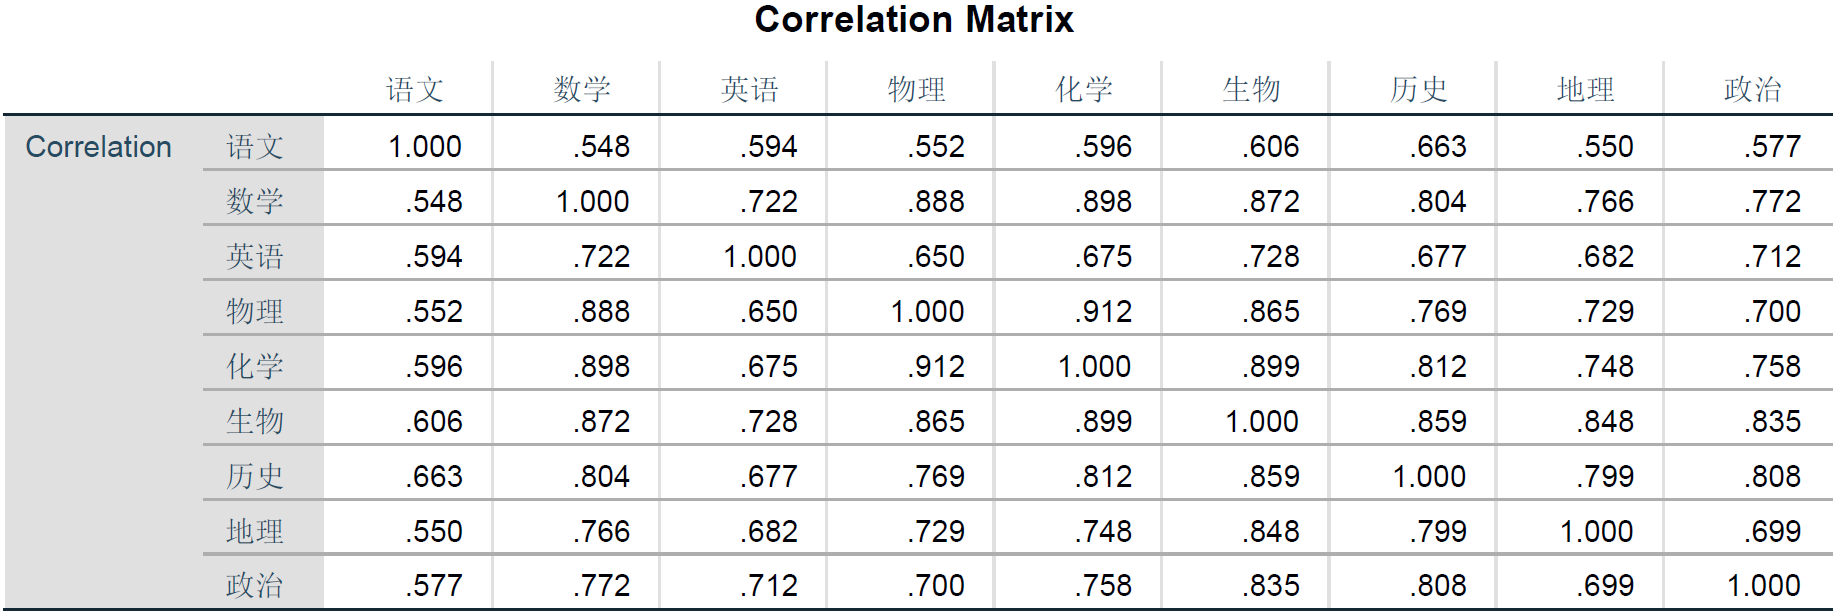
\includegraphics[scale=0.185]{样本相关阵.png}
    \end{center}
    \vspace{-0.5cm}
\end{frame}


\begin{frame}{公因子方差表}
    \begin{center}
        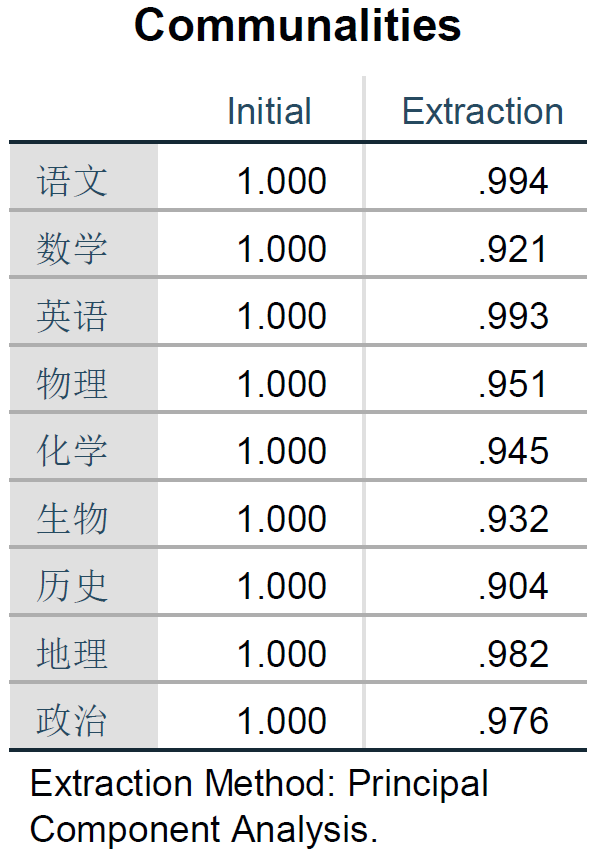
\includegraphics[scale=0.36]{公因子方差表.png}
    \end{center}
    \vspace{-0.5cm}
\end{frame}


\begin{frame}{各个主成分解释原始变量总方差表}
    \begin{center}
        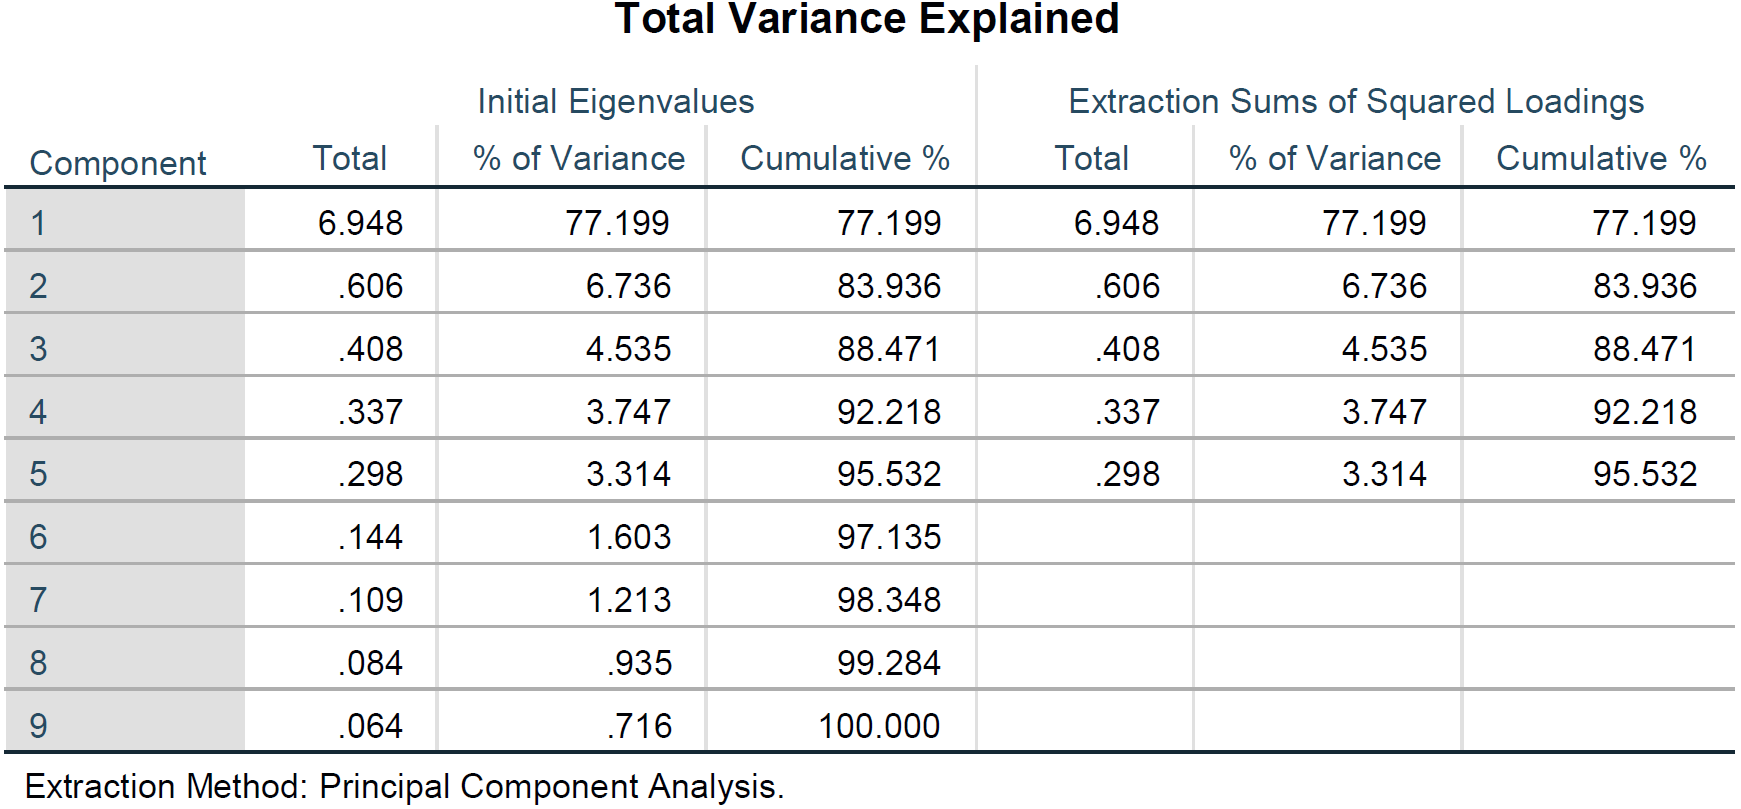
\includegraphics[scale=0.195]{总方差解释表.png}
    \end{center}
    \vspace{-0.5cm}
\end{frame}


\begin{frame}{成分矩阵}
    \begin{center}
        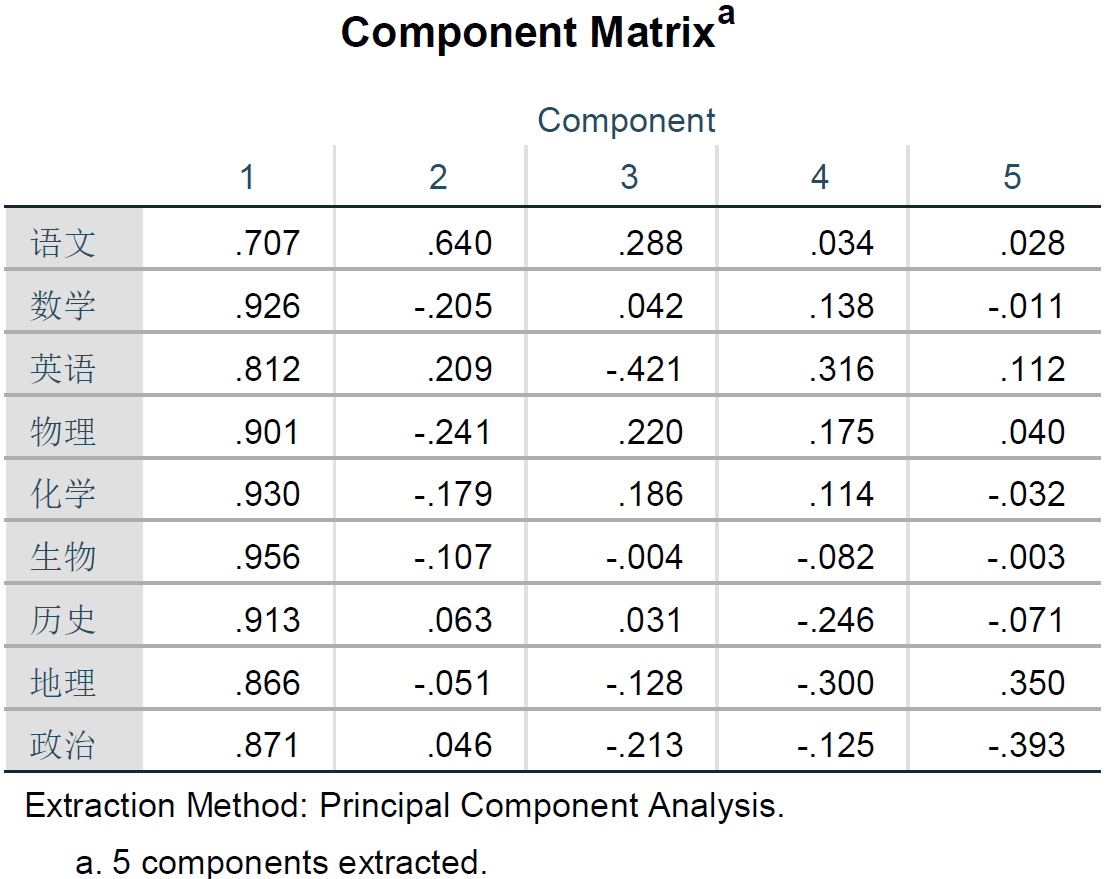
\includegraphics[scale=0.21]{成分矩阵.png}
    \end{center}
    \vspace{-0.5cm}
\end{frame}


\begin{frame}

    \footnotesize
    \begin{align*}
        y_1 &= 0.268x_1+0.351x_2+0.308x_3+0.342x_4+ 0.353x_5+0.363x_6+ 0.346x_7+\\
           &\quad \ \begin{multlined}[t]
            0.329x_8+0.330x_9
           \end{multlined}
    \end{align*}
    
    \begin{align*}
        y_2&=0.822x_1 -0.263x_2 + 0.268x_3 -0.310x_4 -0.230x_5 -0.137x_6 + 0.081x_7 - \\
        & \quad \ \begin{multlined}[t]
            0.066x_8 + 0.059x_9
        \end{multlined}
    \end{align*}

    \begin{align*}
        y_3 &=0.451x_1 + 0.066x_2 -0.659x_3 + 0.344x_4+  0.291x_5 -0.006x_6 + 0.049x_7 - \\
        &\quad \ \begin{multlined}[t]
            0.200x_8 -0.333x_9
        \end{multlined}
    \end{align*}

    \begin{align*}
        y_4 &= 0.059x_1 + 0.238x_2 + 0.544x_3 + 0.301x_4 + 0.196x_5 -0.141x_6 -0.424x_7 - \\
        &\quad \ \begin{multlined}[t]
            0.518x_8 -0.215x_9
        \end{multlined}
    \end{align*}

    \begin{align*}
        y_5 &= 0.051x_1 -0.020x_2 + 0.205x_3 + 0.073x_4 -0.059x_5 -0.005x_6 -0.130x_7 + \\
        & \quad \ \begin{multlined}[t]
            0.641x_8 -0.720x_9
        \end{multlined}
    \end{align*}

\end{frame}

